\chapter{Companding - Redundancy Reduction}
\label{ch:part1}

\section{Companding}

I dette afsnit vil vi gennemgå begrebet `companding`, som en er sammentrækning af `compresseion`og `expansion`. 

Companding er i korte træk en metode til begrænse redundans i talesignaler. Dette gøres ved at transformere talens normale Laplacian distribuerede pdf, om til en mere rektangulær pdf, for derefter kunne kode signalet med en konstant-længde kode. Hos modtageren gendannes signalet til dets oprindelige form. Generelt vinder man 4 bits/sample ved companding, og kan altså ved 8 bit/sample, få et signal der har samme kvalitet som et signal med 12 bit/sample. 

Signalers kvalitet kan objektiv set beskrives ved hjælp af `Signal to Quantization Noise Ratio`, som er altså er et forhold mellem signalets samlede størrelse, og størelsen af den quantiserede signal. 

\section{Analyse af optaget tale}

I dette afsnit vil vi bruge de førnævnte begreber til at analysere et stykke optaget tale. Filen med talen, oak.wav, er samplet med 8 kHz, med 16 bits/sample. Vi lægger ud med at quantize signalet med 12 bit, for at have en reference, som vi kan sammenligne signalet med efter companding. 

 \begin{figure}[!ht]
 	\centering
 	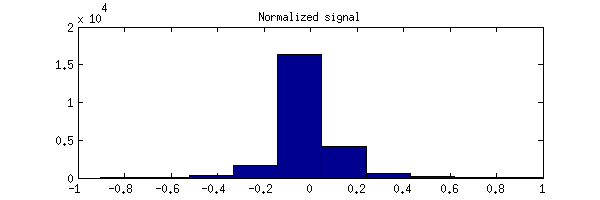
\includegraphics[width=0.8\textwidth]{resources/part1_original}
 	\caption{Pdf for originalt quantized signal}
 	\label{fig:part1_1}
 \end{figure}

 Det originale signal er quantized med 12 bits, hvilket giver en pdf som ses på figur \ref{fig:part1_1}. Som det kan ses er pdf'en ikke særlig rektangulær, men minder derimod meget om en Laplacian distribution. I MATLAB kan vi udregne SQNR til at være $59.22\ dB$. Vores mål med companding er altså at opnå en større SQNR med samme antal bits, eller opnå samme SQNR, med lavere antal bits. 

\subsection{Compression}
Først komprimeres signalet for at opnå en mere rektangulær pdf. Figur \ref{fig:part1_2} viser pdf'en, efter at signalet er blevet compressed med mu-law compression. Det er tydeligt at signalet ikke er blevet fuldstændig rektangulært, men dog meget mere rektangulært end det originale signals pdf. Det er nu på tide at lave en quantization af signalet, i første omgang med 12 bits som referencen.

\begin{figure}[!ht]
	\centering
	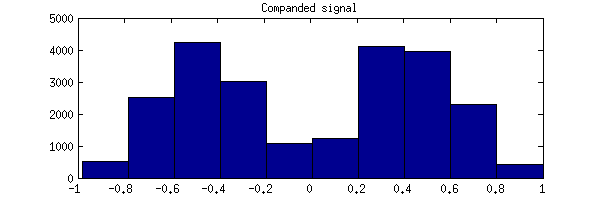
\includegraphics[width=0.8\textwidth]{resources/part1_compressed}
 	\caption{Pdf for compressed signal}
 	\label{fig:part1_2}
\end{figure}

\subsection{Expanding}
Signalet er nu først blevet compressed, og herefter quantized. Det er dermed på tide at expande signalet tilbage til dets oprindelige form. Figur \ref{fig:part1_3} viser pdf'en for signalet efter at det er blevet expanded. I MATLAB udregnes signals SQNR til at være $70.9\ dB$ - SQNR er altså blevet betydelig større. Det er altså muligt at opnå et signal med væsentlig mindre støj, ved hjælp af samme antal bits.

\begin{figure}[!ht]
	\centering
	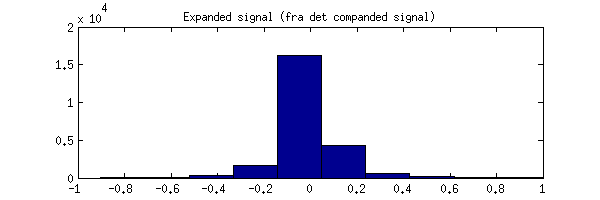
\includegraphics[width=0.8\textwidth]{resources/part1_expanded}
 	\caption{Pdf for expanded signal}
 	\label{fig:part1_3}
\end{figure}

\subsection{Færre bits - samme kvalitet}
Det kunne nu være interessant at undersøge, hvor få bits vi behøver at bruge for at opnå den samme kvalitet som i referencen. 

MATLAB afslører, at ved en quantization ved 10 bits, får vi en SQNR på $58\ dB$. Vi kan altså bruge 2 bits mindre, og stadig opnå tilnærmelsesvis samme kvalitet.




